\chapter{Wykorzystane technologie}

W świecie technologii pierwszym krokiem do osiągnięcia sukcesu przez system jest przyciągnięcie chętnych, którzy będą tworzyć na nią oprogramowanie. Apple dobrze zdaje sobie z tego sprawę, więc robią wszystko aby zjednać sobie programistów i zapewnić im wygodne, funkcjonalne narzędzia. Nie ma żadnych wątpliwości, że iPhone osiągnął sukces między innymi dzięki dostępnym aplikacjom, które bez programistów z pewnością nigdy by nie powstały. Udostępniane przez Apple narzędzia z pewnością są dalekie od ideału, jednakże dostarczają ogromne możliwości dzięki pełnemu pakietowi, z którego pomocą sprawiają, że jedynym ograniczeniem jest wyobraźnia programisty. W tym rozdziale opiszę narzędzia wykorzystane do tworzenia projektu \textbf{EPUBKit}. Są to głównie technologie Apple, co daje pogląd na to jak zaawansowane są ich narzędzia oraz pod koniec rozdziału przedstawiłem dodatkowe biblioteki, które zostały wykorzystane w projekcie.

\section{Xcode i Developer Tools}

\begin{figure}[ht!]
  \centering
  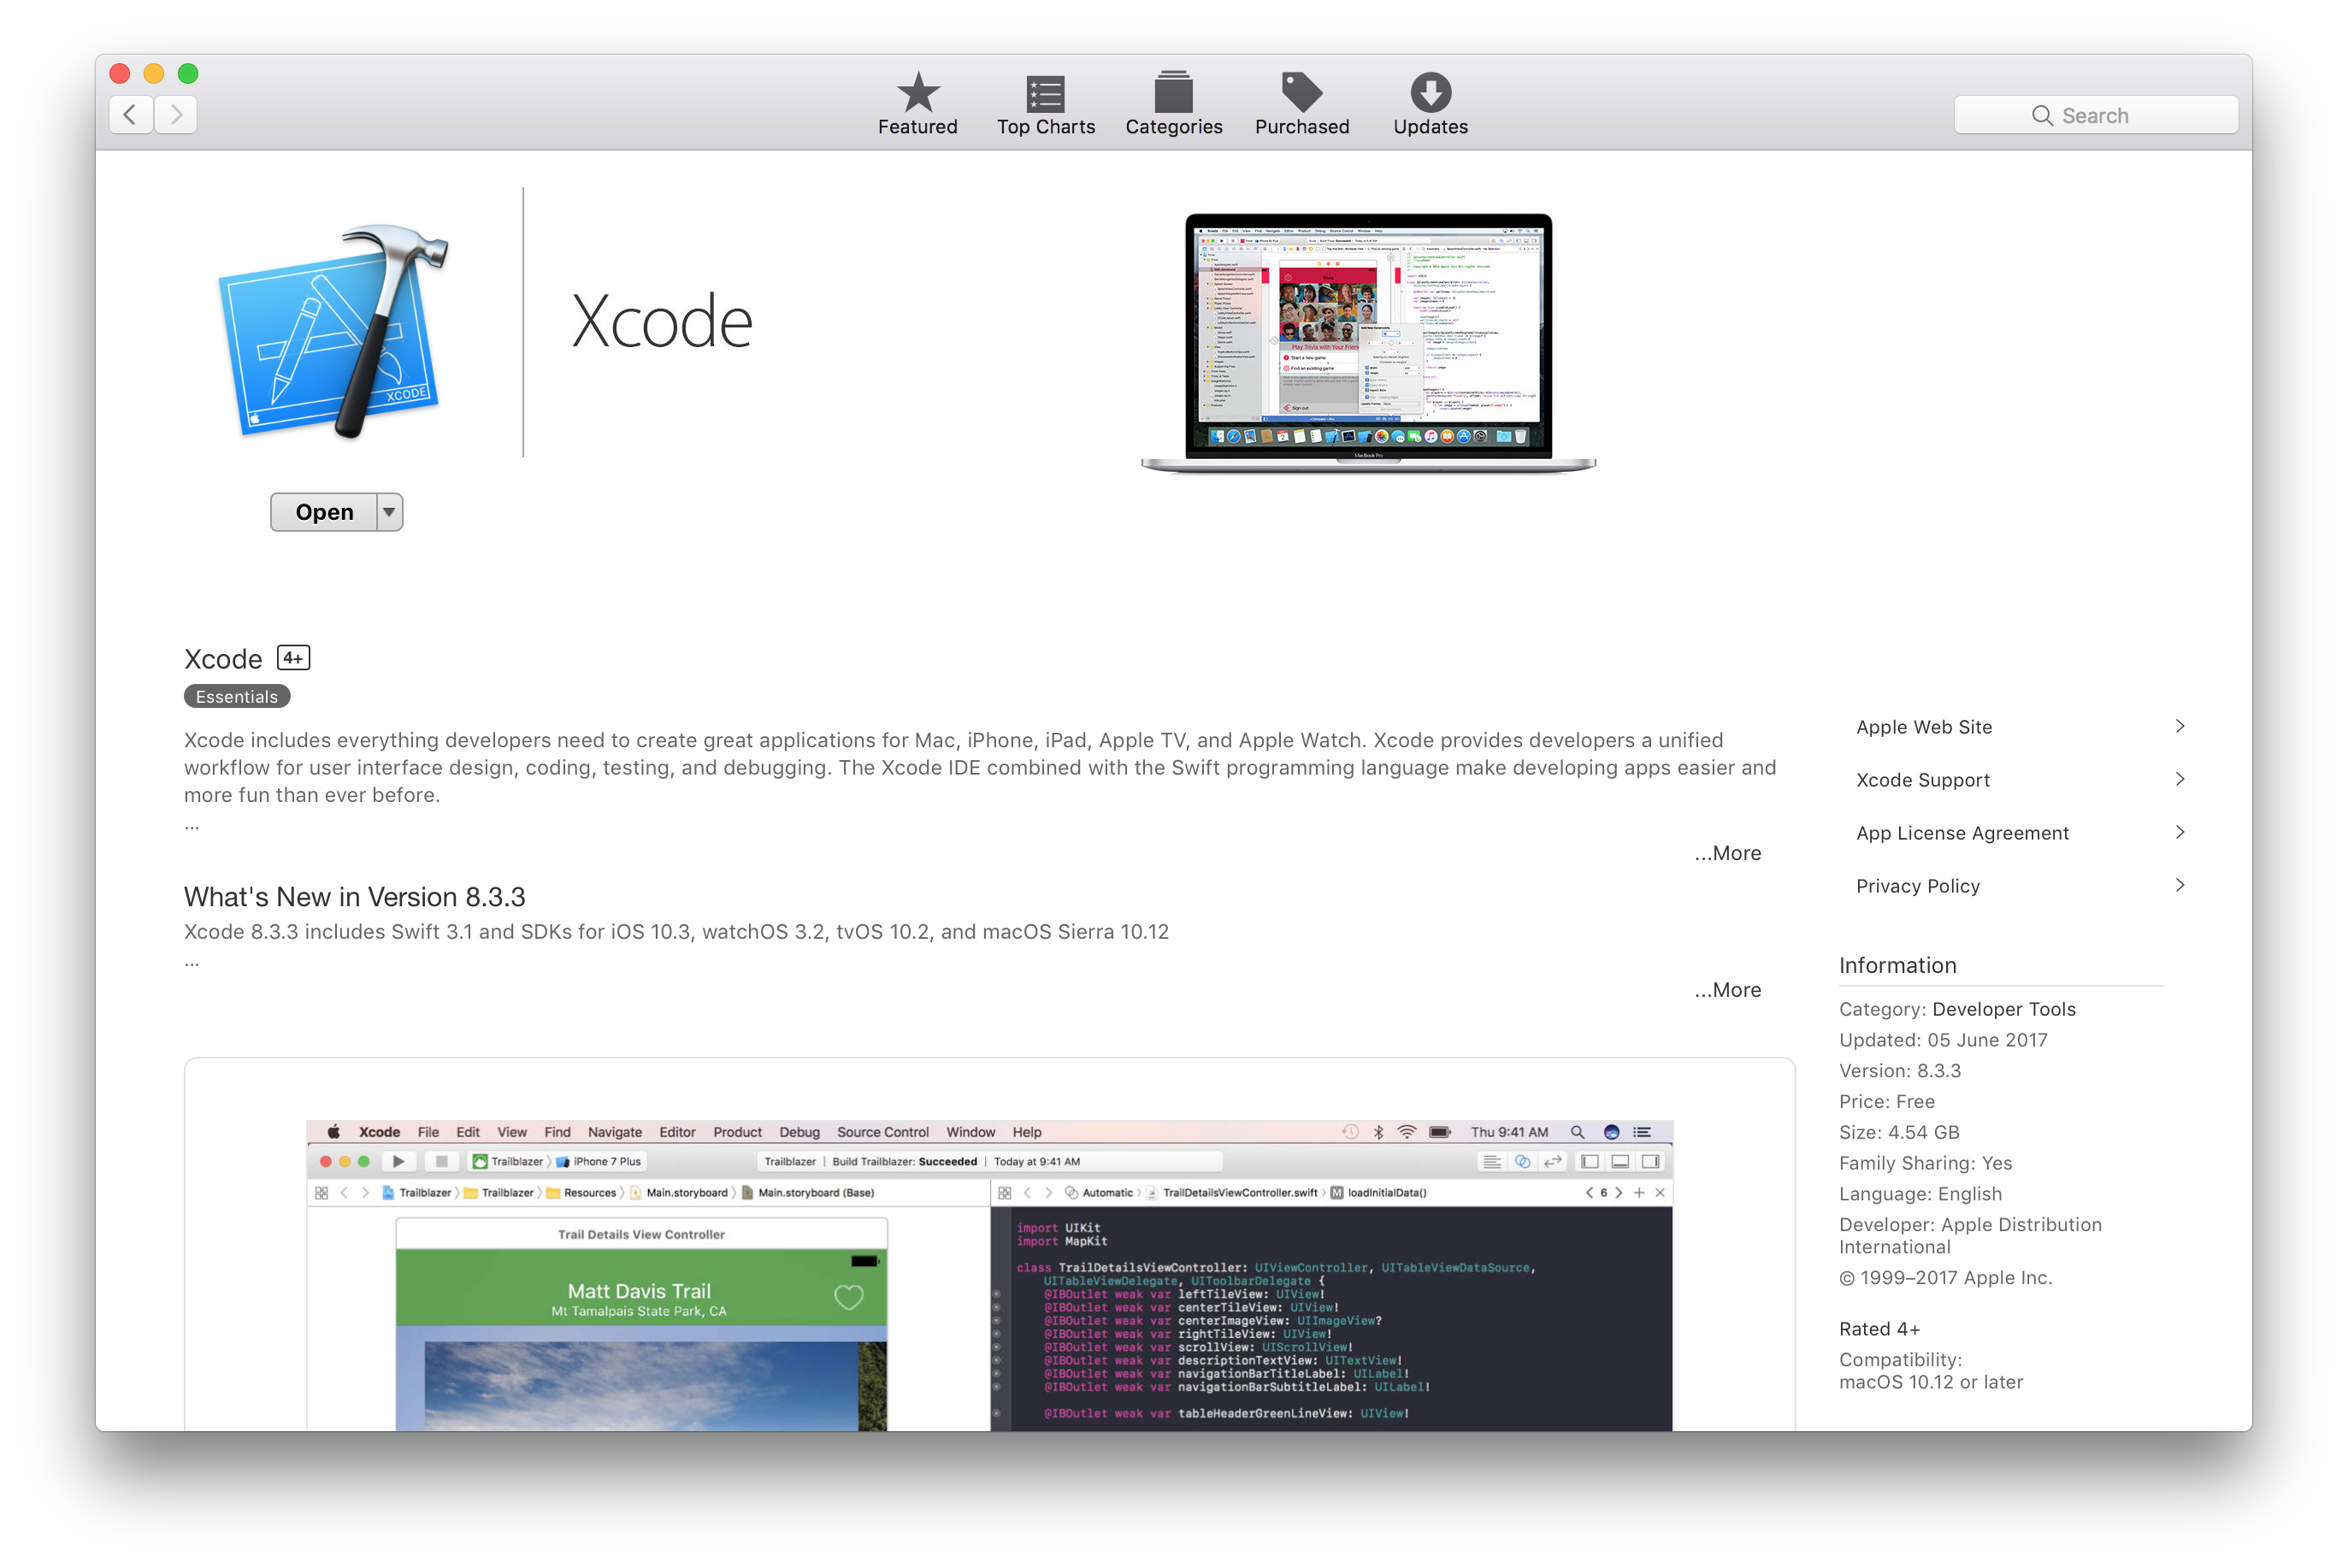
\includegraphics[width=120mm]{images/chapter-2-image-1-appstore.png}
  \caption{Xcode w App Store}
  \label{fig:xcodeappstore}
\end{figure}

Xcode jest IDE (Integrated Development Environment) stworzonym przez Apple i dostępnym za darmo do pobrania z App Store (patrz: rysunek \ref{fig:xcodeappstore}), sklepu z aplikacjami do którego dostęp mają wyłącznie użytkownicy komputerów z systemem Mac OS. Jest wyposażony w pakiet wszystkich narzędzi (Developer Tools) potrzebnych dla programistów, aby tworzyć aplikacje na platformę iOS. Główną aplikacją pakietu jest Xcode IDE, który wraz z wspomagającymi aplikacjami dostępnymi w pakiecie takimi jak Simulator czy Instruments, czyni pracę przy tworzeniu aplikacji płynną i efektowną. W tym rozdziale przedstawię właśnie te narzędzia ze względu na ich rolę w procesie tworzenia aplikacji.

\subsection{Xcode IDE}

Xcode jako nowoczesne, produktywne środowisko jest miejscem w którym programista aplikacji na iOS spędza większość swojego czasu. Całość prac wykonywanych przy produkcji aplikacji może zostać wykonana właśnie tutaj. Najbardziej podstawowy element jakim jest edytor tekstu dobrze współgra z takimi narzędziami jak Interface Builder, który pozwala w prosty sposób zaprojektować stronę wizualną aplikacji przy użyciu \textit{Storyboardów}, a następnie stworzyć referencję w kodzie do wybranych przez nas elementów przez proste przeciągnięcie myszką. Storyboardy są opcjonalnym, aczkolwiek bardzo pożytecznym narzędziem szczególnie dla programistów stawiających swoje pierwsze kroki na tej platformie. Zapewniają one wizualne wyobrażenie interfejsu aplikacji, nad którą wykonywana jest praca, a projektowanie dowolnego widoku, który będzie wyglądał dobrze na każdym urządzeniu w dowolnej orientacji, jest relatywnie proste po zapoznaniu się z kilkoma elementarnymi zasadami. Interface Builder jest widoczny na rysunku \ref{fig:xcodeassistant}, po lewej stronie widoku \textit{Assistant editor} w Xcode.

\begin{figure}[ht!]
  \centering
  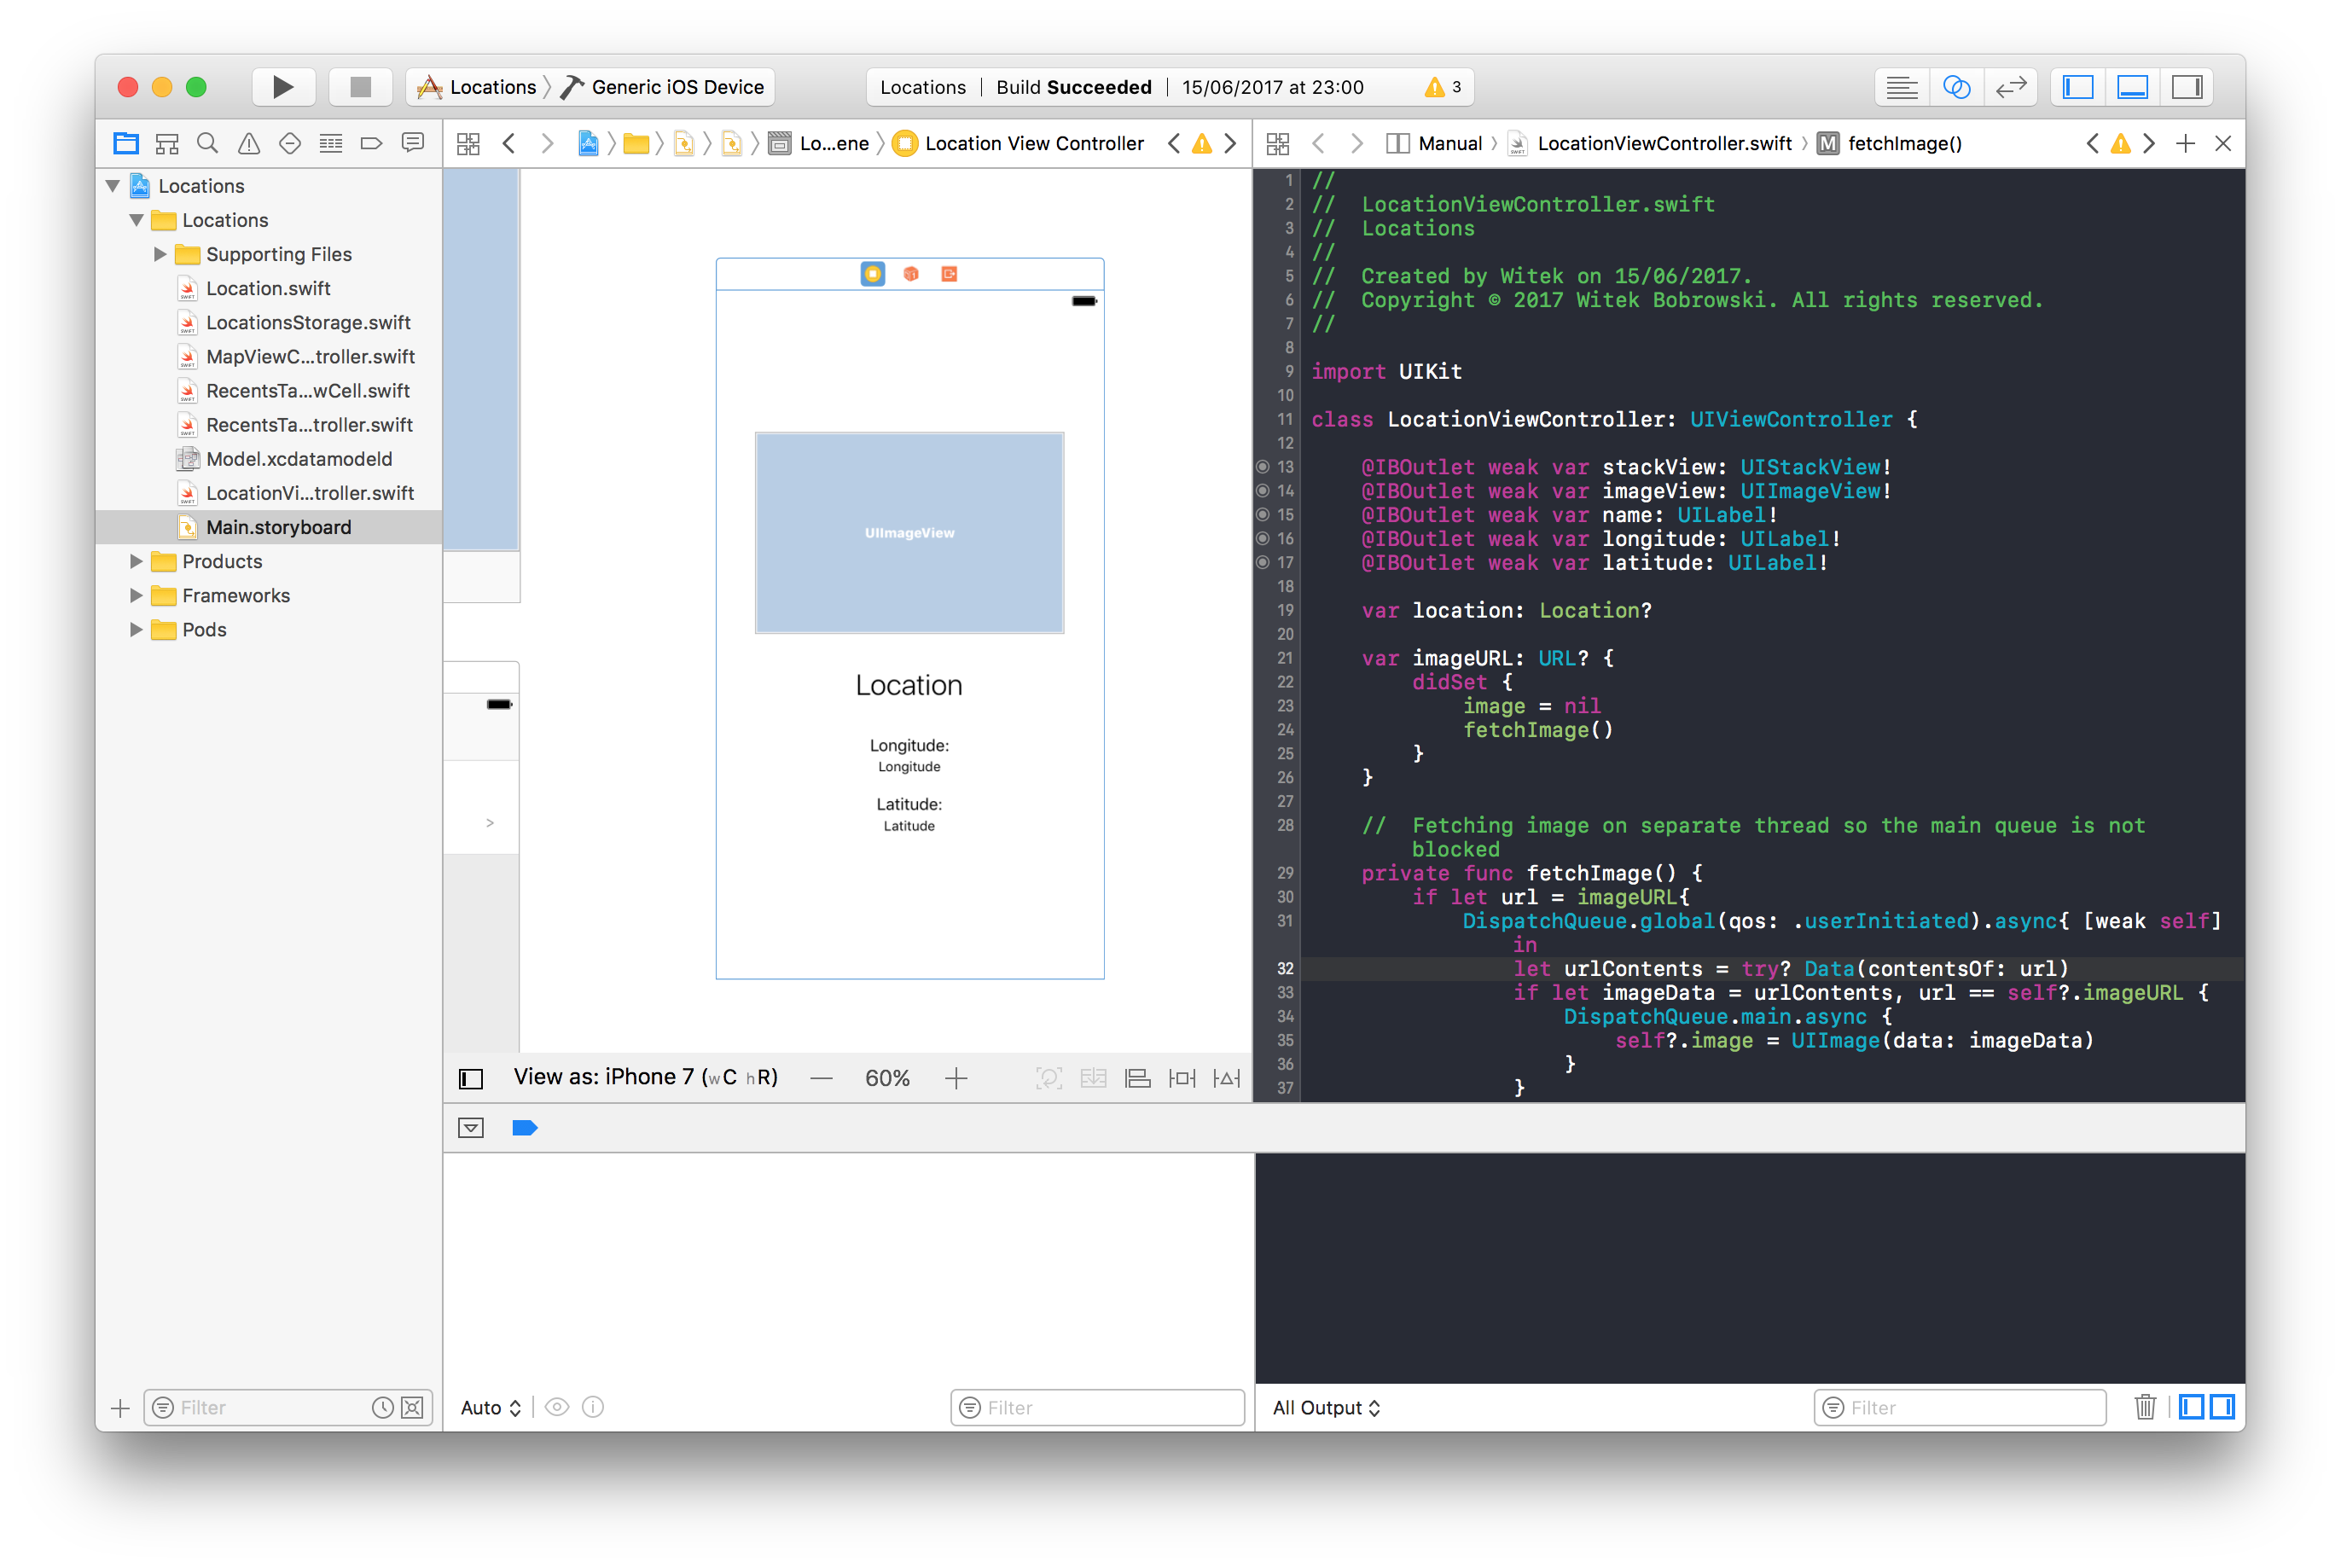
\includegraphics[width=120mm]{images/chapter-2-image-2-xcode.png}
  \caption{Xcode i widok \textit{Assistant editor}}
  \label{fig:xcodeassistant}
\end{figure}

Storyboardy tworzy się w jednym pliku o formacie .storyboard. Dlatego często w profesjonalnej produkcji rezygnuje się z nich ze względu na konflikty w systemach kontroli wersji. Konflikty te powstają w wyniku pracy wielu programistów, a ponieważ plik .storyboard jest w rzeczywistości plikiem XML, który został wygenerowany automatycznie, rozwiązywanie konfliktów bywa kłopotliwe, a przy dużych projektach problematyczne. Dlatego rezygnuje się z nich na rzecz tworzenia widoków tylko przy użyciu kodu, oraz niezależnych plików \textit{Xib}. Pliki te pozwalają na ustawienie elementów w stylu znanym ze Storyboardów, lecz w przeciwieństwie do nich reprezentują pojedynczy widok, dzięki czemu można uniknąć konfliktów, a jednocześnie tworzenie bardziej skomplikowanych widoków jest znacznie ułatwione. Xcode zapewnia wsparcie dla systemu kontroli wersji git. Przy tworzeniu nowego projektu, gdy jest o to poproszony, inicjalizuje nowe repozytorium. Dodatkowo w nawigatorze projektu, w którym widać jego strukturę, Xcode oznaczy literą \textit{M} pliki które git oznacza jako pliki w których dokonano zmian (modified), a literą \textit{A} pliki które zostały dodane (new file) od czasu poprzedniego zachowania zmian.
W najnowszej wersji 9.0, Xcode zyskał nową funkcjonalność -- Source Control Navigator, który pozwala na eksplorowanie poszczególnych gałęzi repozytorium i podglądu dowolnego momentu w jego historii.

\subsection{Simulator}

Simulator pozwala na uruchomienie zbudowanej aplikacji na dowolnym urządzeniu z iOS, które jest w stanie symulować. Gdy chce się przetestować aplikację wystarczy w pasku narzędzi Xcode wybrać dowolny model urządzenia, które chcemy symulować, tak jak przedstawiono to na rysunku \ref{chapter-2-image-3-target}. Oprócz telefonów iPhone znajdują się tam również tablety iPad. Jeżeli podłączymy do komputera fizyczne urządzenie, Xcode również je wykryje i pozwoli na zainstalowanie i uruchomienie na nim aplikacji. W kolejnym kroku Xcode przejdzie to etapu budowania aplikacji, w którym kompiluje pliki źródłowe, a następnie umieści aplikację w symulatorze wybranego przez nas urządzenia, co jest widoczne na rysunku \ref{chapter-2-image-4-simulator}.

\begin{figure}[ht!]
\centering
\begin{subfigure}{.5\textwidth}
  \centering
  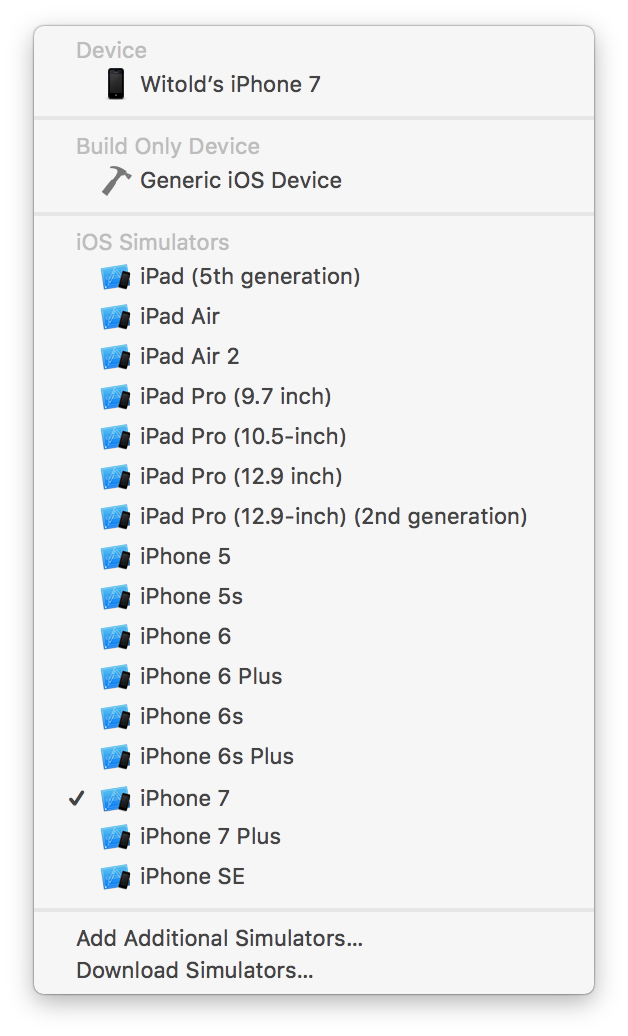
\includegraphics[width=.4\linewidth]{images/chapter-2-image-3-target.png}
  \caption{Wybór docelowego urządzenia}
  \label{chapter-2-image-3-target}
\end{subfigure}%
\begin{subfigure}{.5\textwidth}
  \centering
  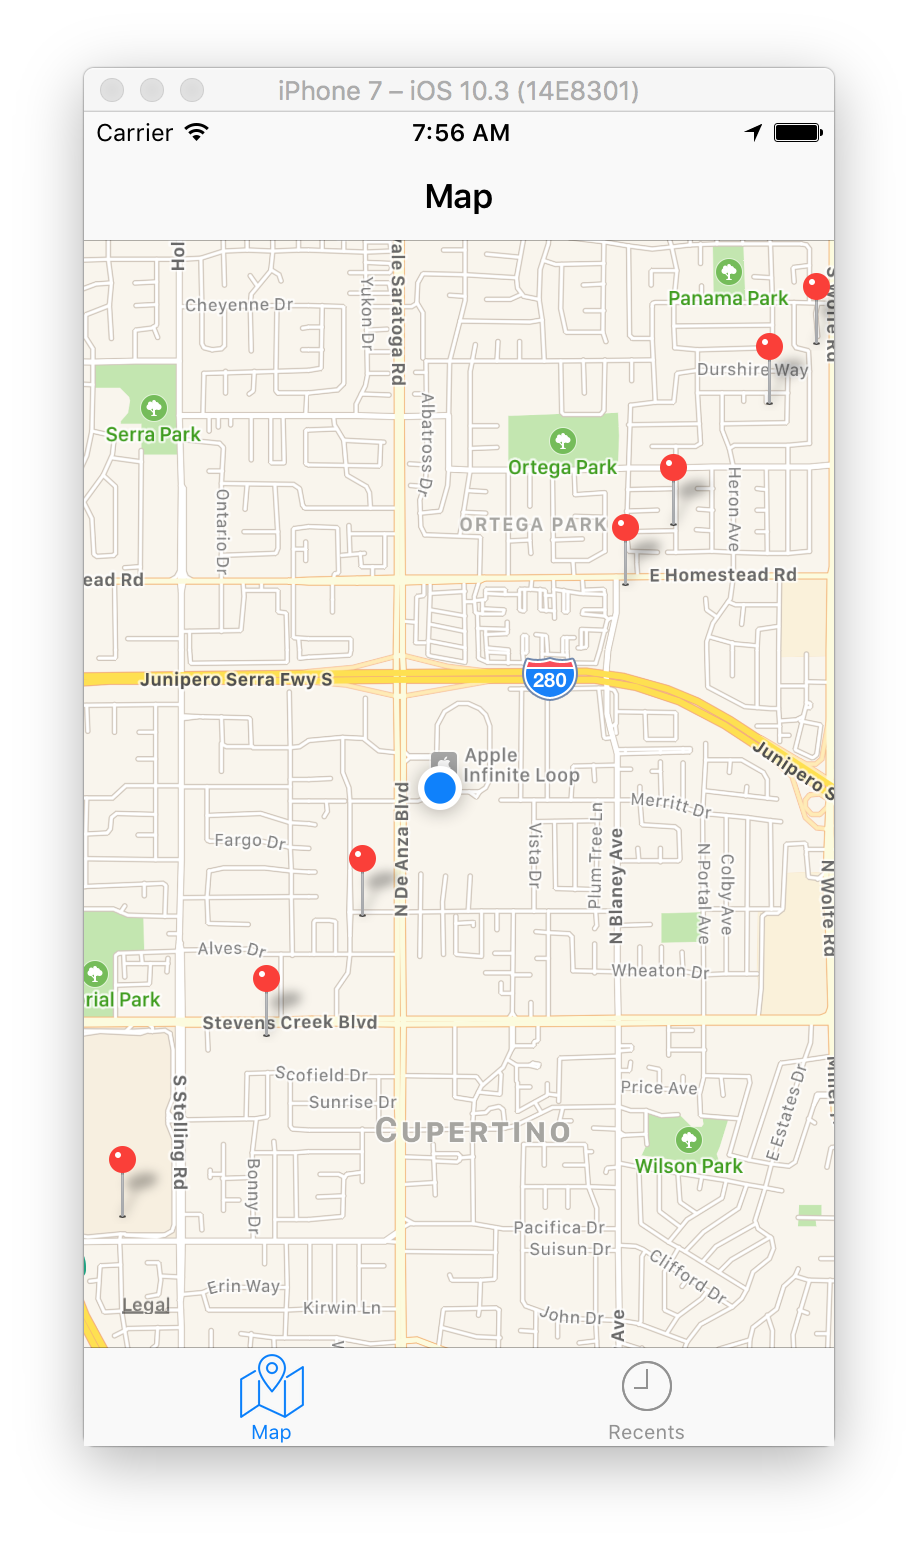
\includegraphics[width=.4\linewidth]{images/chapter-2-image-4-simulator.png}
  \caption{Uruchomiona aplikacja na iPhone 7}
  \label{chapter-2-image-4-simulator}
\end{subfigure}
\caption{Po wybraniu urządzenia w Xcode, Simulator uruchamia na nim aplikację}
\label{chapter-2-image-4-5}
\end{figure}

Podczas gdy aplikacja jest uruchomiona i testowana na symulatorze, Xcode pozwala na podgląd użycia zasobów takich jak procesor, pamięć RAM, pamięć dyskowa oraz sieć. Po wybraniu dowolnego z wyżej wymienionych zasobów z nawigatora \textit{Debuggera} ukazuje nam się bardziej szczegółowy podgląd na to, w jakim stopniu aplikacja obciąża urządzenie, co pozwala na szczegółowe testowanie (patrz: rysunek \ref{fig:simulatorcpu}).

\begin{figure}[ht!]
  \centering
  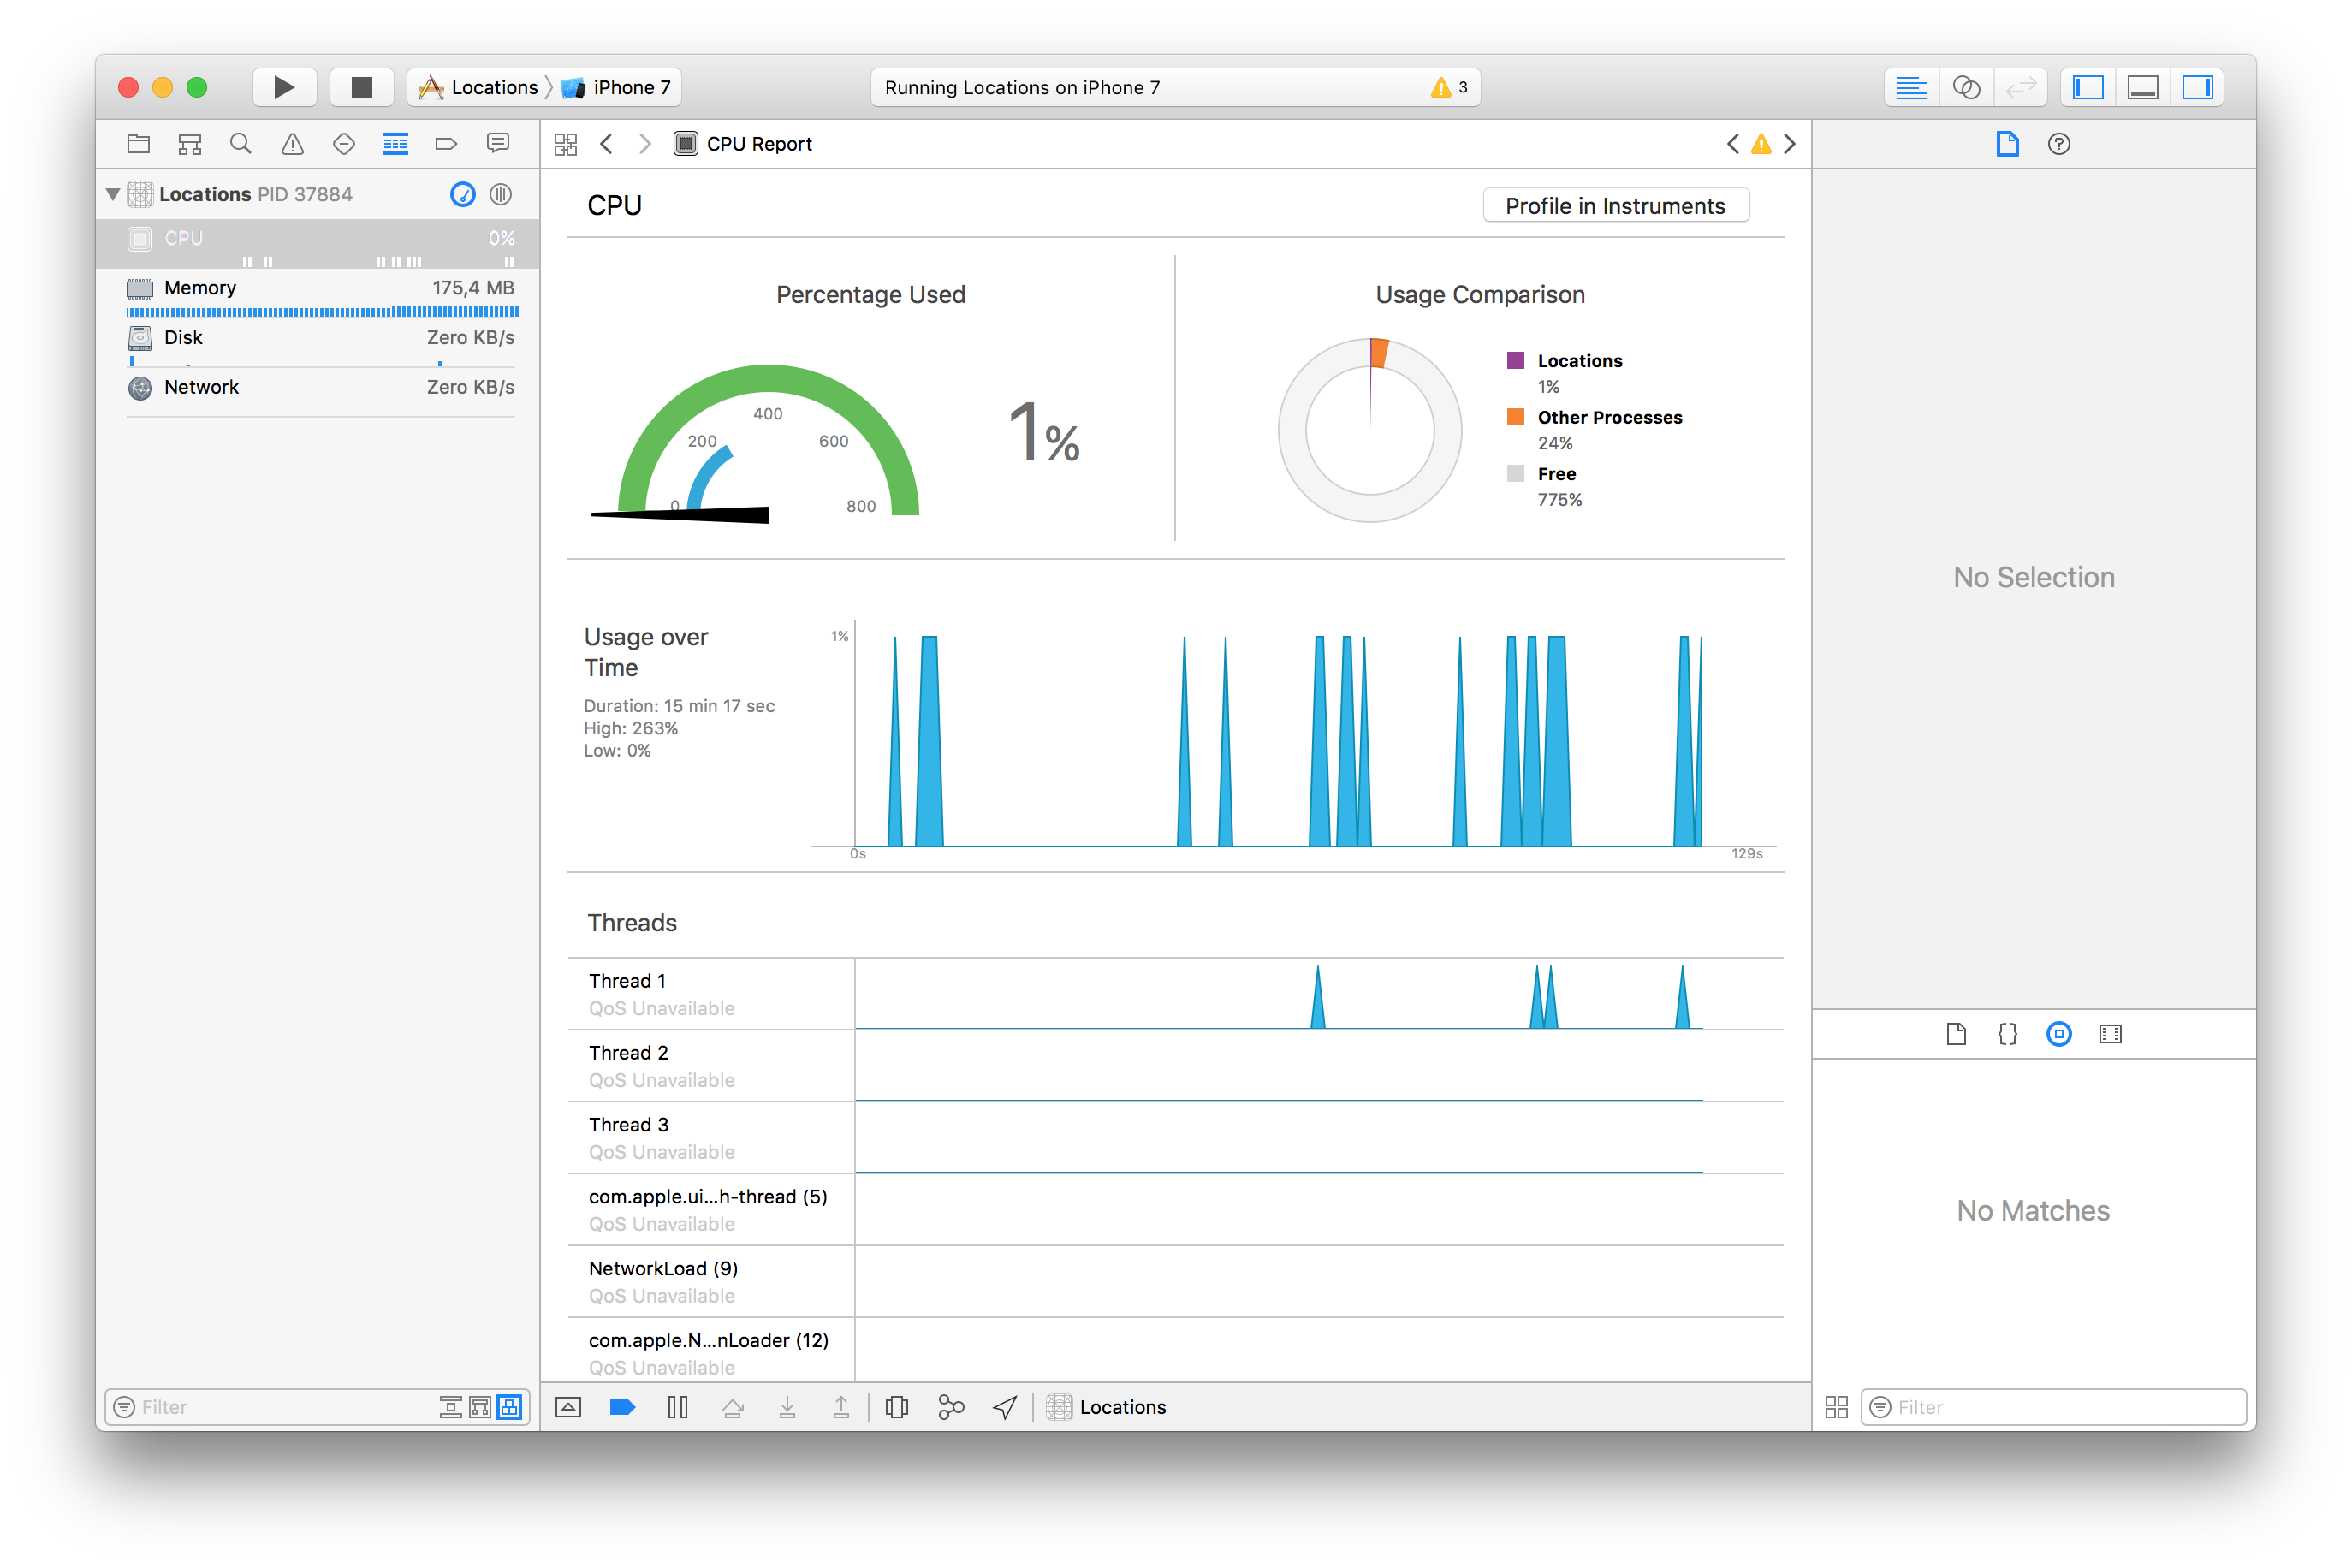
\includegraphics[width=120mm]{images/chapter-2-image-5-debugger.png}
  \caption{Użycie CPU na symulatorze odświeżane na bieżąco i wyświetlone w Xcode}
  \label{fig:simulatorcpu}
\end{figure}

\subsection{Instruments}

Widok poboru zasobów w Xcode jest bardzo pomocny na poglądową ocenę wydajności naszej aplikacji. Jeżeli jednak chcemy poddać ją prawdziwej próbie, musimy uruchomić kolejne narzędzie jakim jest Instruments. Instruments widoczne na rysunku \ref{fig:instruments} jest aplikacją, dzięki której dokonamy pomiaru nie tylko każdego zasobu na urządzeniu, ale również dostajemy możliwość nadzoru takich aktywności jak alokowanie pamięci dla obiektów, zmiany layoutu widoków czy zmiany w Core Data, natywnej bazie danych dla iOS.

Niezależnie od tego jak szybkie i wydajne są w dzisiejszych czasach telefony, optymalny kod nadal jest podstawą prawidłowego działania aplikacji i niedbałe projektowanie architektury może być fatalne w skutkach. Cykle referencji mogą powodować niechciane wycieki pamięci, a problemy powstające podczas przerysowywania się widoków spowodują nieczytelny interfejs. Jeżeli takie błędy nie zostaną wykryte na etapie produkcyjnym, a dogłębne testy aplikacji nie zostaną przeprowadzone przed oddaniem jej do recenzji, aplikacja najprawdopodobniej zostanie odrzucona, co wiąże się z dodatkowymi opóźnieniami. Aby nasza aplikacja mogła znaleźć się w sklepie AppStore i być dostępna dla każdego, musi ona otrzymać pozytywną recenzje Apple. Pakiet narzędzi dostarczanych przez Apple spełnia swoje zadanie i dla większości programistów są one wystarczające. Istnieją rozwiązania firm trzecich, JetBrains dostarcza alternatywne IDE do produkcji aplikacji -- AppCode, które cieszy się bardzo dobrą reputacją wśród użytkowników.

\begin{figure}[ht!]
  \centering
  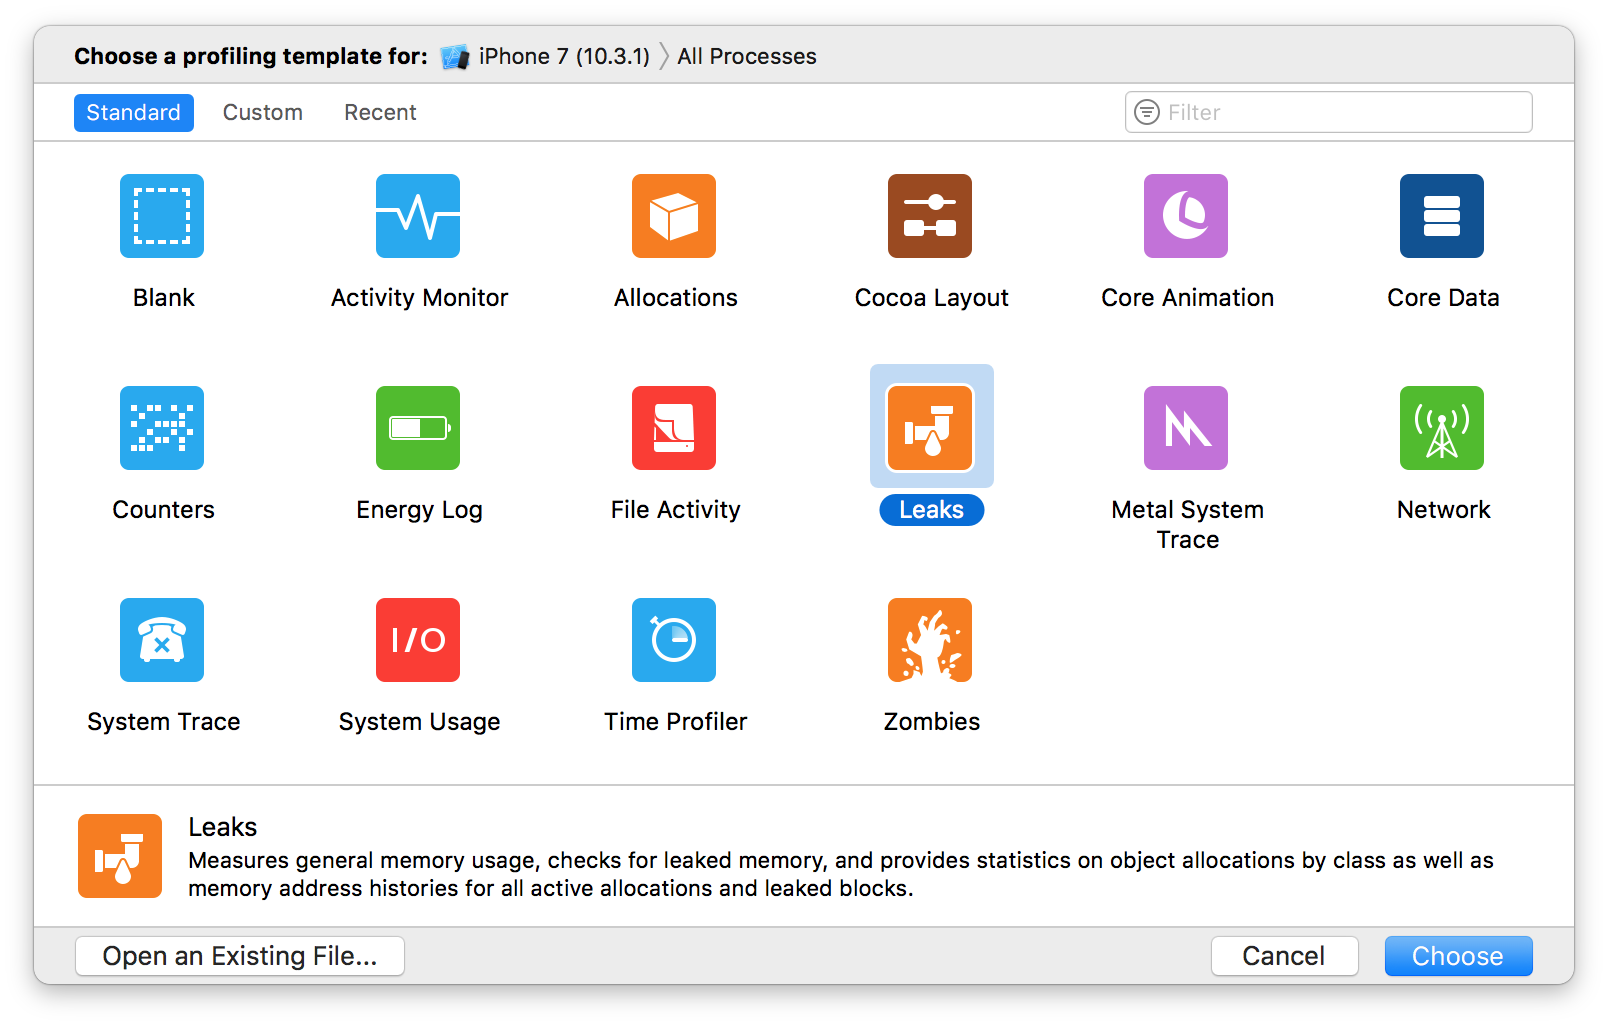
\includegraphics[width=120mm]{images/chapter-2-image-6-instruments.png}
  \caption{Instruments, widok menu głównego}
  \label{fig:instruments}
\end{figure}

\section{Swift}

Gdy w 1996 roku Apple przejęło NeXT wraz z ich oprogramowaniem, Objective-C stało się głównym językiem do tworzenia oprogramowania na najnowszy system operacyjny OS X. Wraz z OpenStepem Apple znalazło się w posiadaniu takich narzędzi jak Interface Buildier oraz Project Buildier, które z biegiem czasu ewoluowały w Xcode, który znamy dzisiaj. Objective-C służył programistom przez wiele lat, na początku tym tworzącym aplikacje desktopowe, a od ukazania się pierwszego iPhone'a, programistom mobilnym. Objective-C jest bardzo mocno rozwiniętym językiem, co zważając na jego wiek nie powinno nikogo dziwić. Jednak jako język, którego początki sięgają wczesnym latom osiemdziesiątym dwudziestego wieku, z biegiem lat postarzał się, co bardzo upraszczając można by przedstawić stwierdzeniem, iż nie jest wystarczająco nowoczesny.

Twórca LLVM (Low Level Virtual Machine) Chris Lattner\cite{LLVM}, w 2010 roku rozpoczął prace nad nowym językiem, który z założenia miał czerpać inspirację z takich języków jak Objective-C, Haskell, Python czy Ruby. Cztery lata później, Apple na WWDC (Worldwide Developer Conference) zaprezentowało Swifta i wypuściło wersję beta\cite{2014-wwdc-swift}. Swift jest bezpiecznym, szybkim językiem, który agreguje wiele paradygmatów znanych z innych nowoczesnych języków. Jego najważniejszymi cechami są:
\begin{itemize}
    \item automatycznie zarządzana pamięć,
    \item typ opcjonalny, który zapewnia wsparcie dla /textit{nullowych} wskaźników,
    \item zaawansowana obsługa błędów, która zapewnia kontrolowane wyjście z niespodziewanych niepowodzeń,
    \item zmienne, które zawsze są zainicjalizowane przed użyciem,
    \item silne typowanie które po połączeniu z nowoczesną, lekką składnią czyni go językiem zarówno potężnym jak i łatwo dostępnym.
\end{itemize}
Dynamiczny rozwój zawdzięcza inżynierom z Apple oraz społeczności open-source, którzy bardzo intensywnie pracują dodając nowe elementy, naprawiając niedoskonałości oraz optymalizując jego architekturę. Swift dzisiaj jest jednym z najbardziej lubianych języków programowania. Jego popularność wciąż rośnie, a odkąd stał się projektem open-source'owym oprócz systemów Apple, zaczyna być używany do takich celów jak tworzenie aplikacji internetowych. Zdominował platformę iOS i zdetronizował Objective-C, stając się językiem pierwszego wyboru. Wszystkie powstające aplikacje są obecnie tworzone przy jego użyciu, i wiele napisanych w Objective-C jest dzisiaj przepisywanych na nowy język. Warto wspomnieć, że kod w Objective-C i kod w Swiftcie może być użyty w tej samej aplikacji, dzięki czemu może się tam znaleźć również C i C++. Jednak, aby użyć kodu napisanego w C czy w C++ w Swiftcie musimy go najpierw opakować, aby był dla niego dostępny. W przypadku Objective-C, Swift ma dostęp do jego obiektów oraz może dziedziczyć z jego klas. A to zapewnia nam dostęp do wszystkich natywnych bibliotek, czyniąc Swift pełnoprawnym językiem i narzędziem gotowym do użytku już w dniu jego premiery. W projekcie wykorzystano Swift w wersji 3.1.

\section{iOS SDK}

Jak już wspomniano wcześniej, iOS dziedziczy wiele po systemie macOS. W skład iOS SDK wchodzą biblioteki znane już od wielu lat oraz biblioteki stworzone z myślą o urządzeniach mobilnych. W tej sekcji omówiono pokrótce framework CocoaTouch, który dostarcza elementy interfejsu będące podstawą każdej aplikacji i zapewniające wizualną spójność platformy.

\subsection{CocoaTouch}

CocoaTouch jest potomkiem frameworku Cocoa dostępnego na systemach macOS, który jest rozszerzony o interfejs obsługi narzędzi dostępnych w urządzeniu mobilnym takich jak rozpoznawanie gestów, serwis lokalizacji czy obsługa kamery. W skład CocoaTouch wchodzą między innymi biblioteki Foundation, UIKit, MapKit, EventKit i wiele innych. Dzięki temu pakietowi Apple zdefiniowało jak powinny być tworzone aplikacje na iOS. Dostarczony jest zbiór wielu elementów interfejsu użytkownika, które można dowolnie rozszerzać i modyfikować, aby stworzyć unikalny wygląd aplikacji trzymając się wytycznych wyznaczonych przez Apple. Dostęp do gestów zapewni naszej aplikacji lekkość obsługi oraz intuicyjność, a niezliczona ilość innych bibliotek wchodzących w skład CocoaTouch sprawi, że aplikacja nabierze życia. Implementowanie funkcjonalności staje się bardzo proste dzięki wysoko poziomowym interfejsom dającym dostęp do poszczególnych elementów systemu oraz fizycznego urządzenia. CocoaTouch jest najbardziej elementarnym frameworkiem na iOS, ponieważ to on zapewnia na poziomie podstawowym to co potrzebne do stworzenia funkcjonalnej aplikacji. Zakładając że aplikacja powinna agregować, w jakiś sposób przetwarzać, a następnie wyświetlić w odpowiedniej formie zbiór pewnych danych, CocoaTouch w parze ze Swiftem to zagwarantują, oczywiście do pewnego stopnia. W większości przypadków, gdy potrzebujemy wykonać jakieś specyficzne zadanie, lub chcemy je po prostu uprościć unikając implementacji własnego rozwiązania problemu, co było by czasochłonne, będziemy skłaniać się ku zewnętrznym bibliotekom.

\section{Zewnętrzne biblioteki}

Biblioteki te, tworzone przez środowiska open-source’owe, pojedynczych programistów czy wielkie korporacje dadzą nam to czego nie otrzymaliśmy wraz z natywnymi frameworkami. Przykładem jest projekt który opisuje ta praca. Rozwiązuje problem programisty tworzącego własną aplikację, który nie chce tracić czasu na implementowanie funkcjonalności, która zajęła by mu relatywnie dużo czasu, a która niekoniecznie jest głównym celem jego aplikacji. Istnieje wiele sposobów na rozszerzenie naszej aplikacji o wybrane moduły, które bardziej szczegółowo zostaną opisane pod koniec czwartego rozdziału podczas omawiania możliwościach dystrybucji biblioteki. W tej sekcji przedstawiono biblioteki wykorzystane do projektu EPUBKit, które nie wchodzą w skład iOS SDK, a zostały udostępnione do publicznego użytku.

\subsection{Zip}

Zip jest swiftową biblioteką open-source dostępną na licencji MIT, której kod źródłowy znajdziemy na GitHubie \footnote{Adres url: \href{https://github.com/marmelroy/Zip}{github.com/marmelroy/Zip}}. Zip jest narzędziem do archiwizowania plików oraz rozpakowywania archiwów. Wspiera on formaty archiwów .zip, .cbz oraz daje możliwość dodania rozszerzenia pliku który chcemy rozpakować. W przypadku tego projektu dodano format .epub, aby rozpakować książkę elektroniczną w tym właśnie formacie. Zip bazuje na narzędziu minizip napisanym w języku C, również na wolnej licencji, oraz dostępnym na portalu GitHub. Dzięki bibliotece zip, parser biblioteki EPUBKit może w prosty sposób otrzymać dostęp do struktury plików publikacji elektronicznej. Szczegółowe opisanie wykorzystania biblioteki Zip znajduje się w czwartym rozdziale podczas omawiania kodu źródłowego parsera.

\subsection{AEXML}

Kolejną wykorzystaną biblioteką jest AEXML, prosty i lekki parser XML, dostępny publicznie na licencji MIT, również udostępniony na GitHubie\footnote{Adres url: \href{https://github.com/tadija/AEXML}{github.com/tadija/AEXML}}. Ze względu na strukturę elektronicznej publikacji EPUB, parser XML jest niezbędny do rozpoznania zawartości całej struktury dokumentu, identyfikacji elementów oraz określenia ich lokalizacji. AEXML jest swiftowym frameworkiem, a jego API jest czytelne i proste w wykorzystaniu, dzięki czemu idealnie spełnia swoje zadanie w projekcie który opisuje ta praca.
